\section{System Integration}
Since it was known ahead of time that the receiver was to be fully integrated together, a lot of effort was put towards perfecting input and output matching to guarantee maximum power transfer across components. The LNA input, VCO output, and Mixer output are all matched to 50 $\Omega$. The LNA output and Mixer signal input are matched to 500 $\Omega$, we found this to help improve the gain of the Mixer. Since all of the components were matched properly, full system integration was as simple as placing the components together (Fig. ~\ref{fig:fullsystem}). 

\begin{figure}[h]
   \centering
    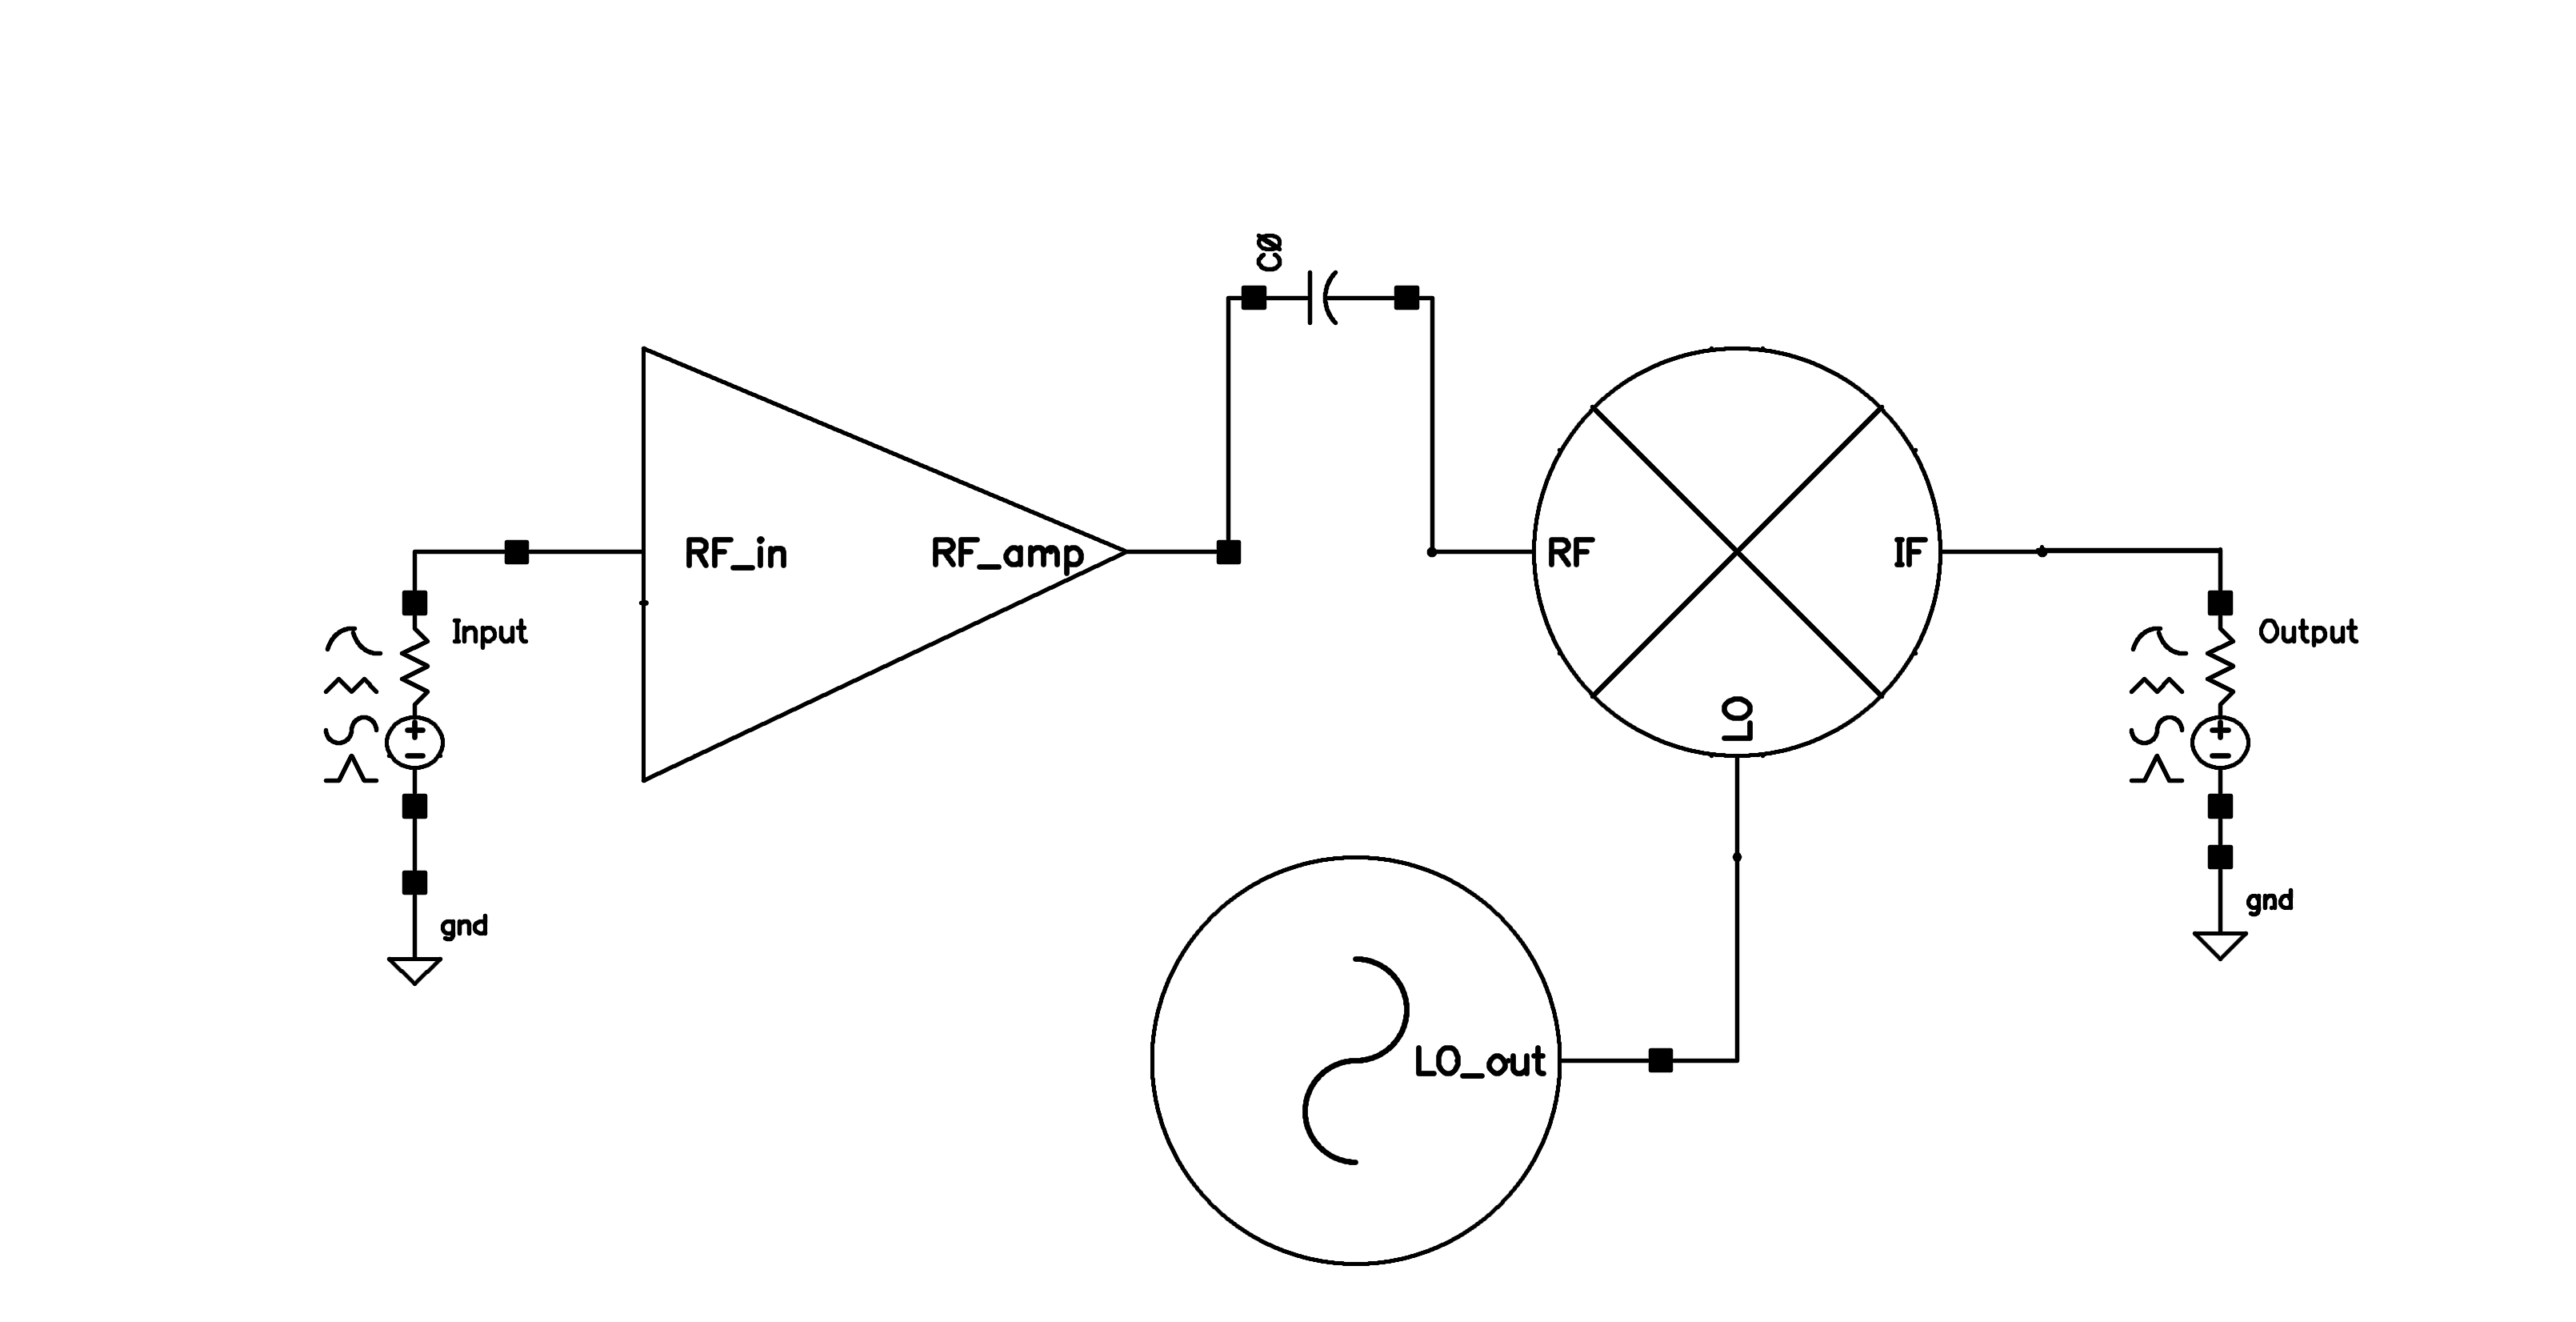
\includegraphics[width=0.5\textwidth]{figures/FullSystem.png}
    \caption{Full system circuit integration, comprised of a Low Noise Amplifier, Mixer, and Voltage Controlled Oscillator. Coupling capacitors are used to remove the DC offset from the LNA. }
    \label{fig:fullsystem}
\end{figure}

In order to test the system, a transient analysis was preformed. An initial input signal of 1mV at 403.5MHz was used to test the system. Fig. ~\ref{fig:fullsystemtrans} shows a clean output response from the system that swings from 55mV to -70mV at 3.5MHz. This leads to an overall swing of 62.5mV, therefore the conversion gain of the entire system is $20log(\frac{62.5mV}{1mV})$ or {\bf 35.92 dB}.

\begin{figure}[h]
   \centering
    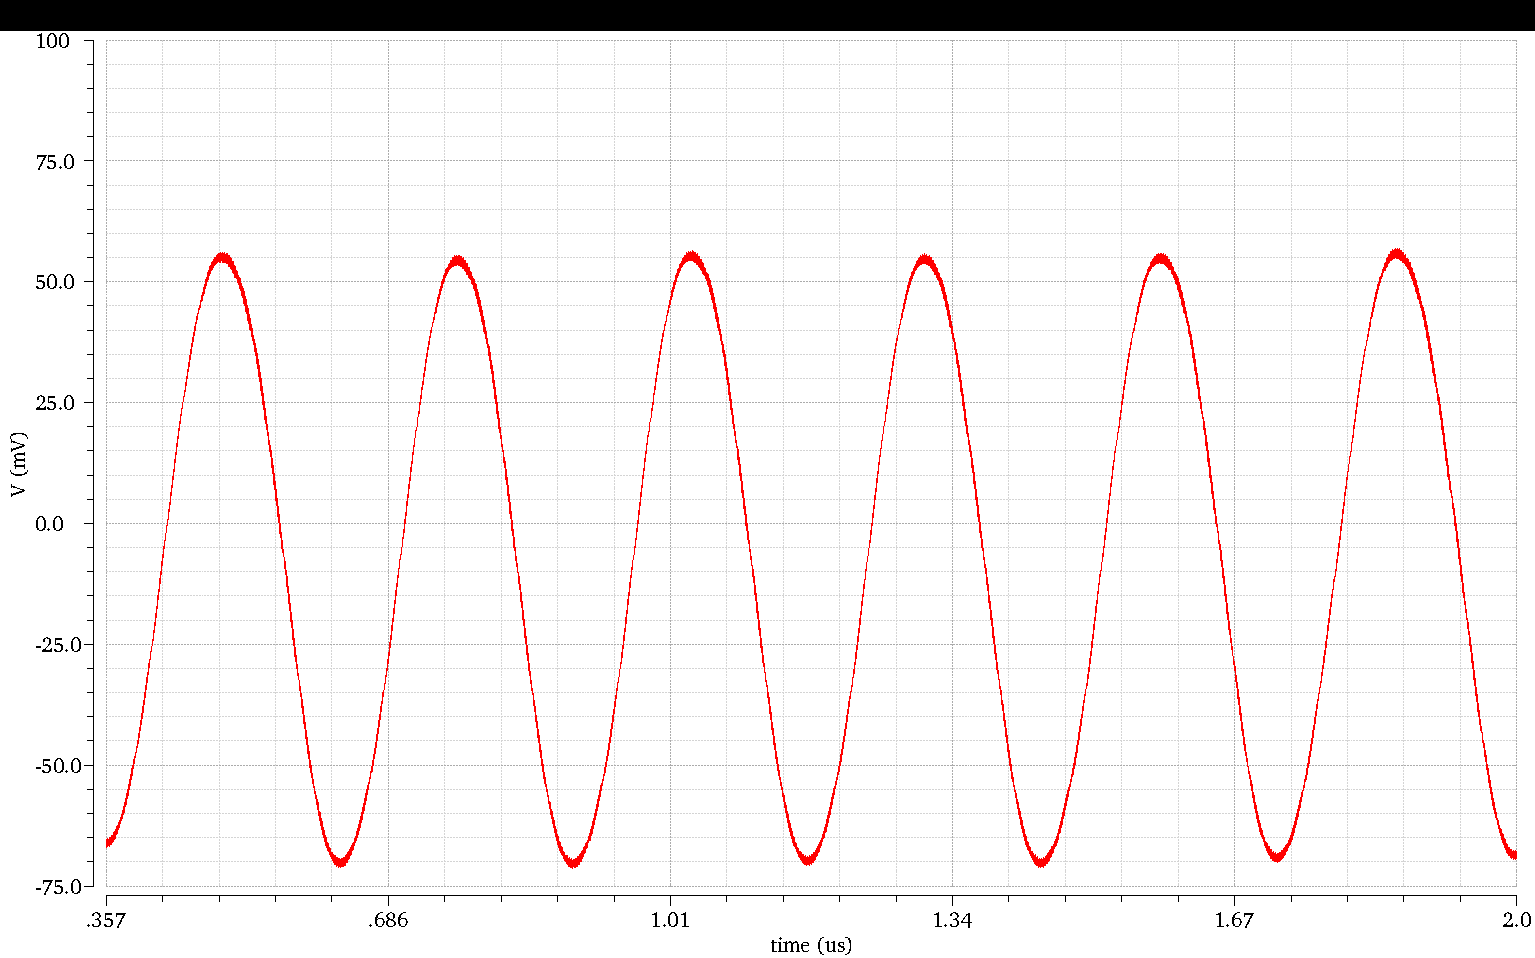
\includegraphics[width=0.5\textwidth]{figures/FullSystemTrans}
    \caption{Transient response of receiver after 357ns startup time}
    \label{fig:fullsystemtrans}
\end{figure}

In order to measure the noise figure, the oscillator was removed and an ideal source was used instead. Although the oscillator in theory would contribute slightly to the noise, it was determined that due to its low LO-IF feed-through that the oscillator has a negligible effect to the total noise. Fig. ~\ref{fig:fullsystemnoise} shows the total noise of the system, at the corner frequency of the output, it was determined that the total noise was {\bf 3.65 dB}.

\begin{figure}[h]
   \centering
    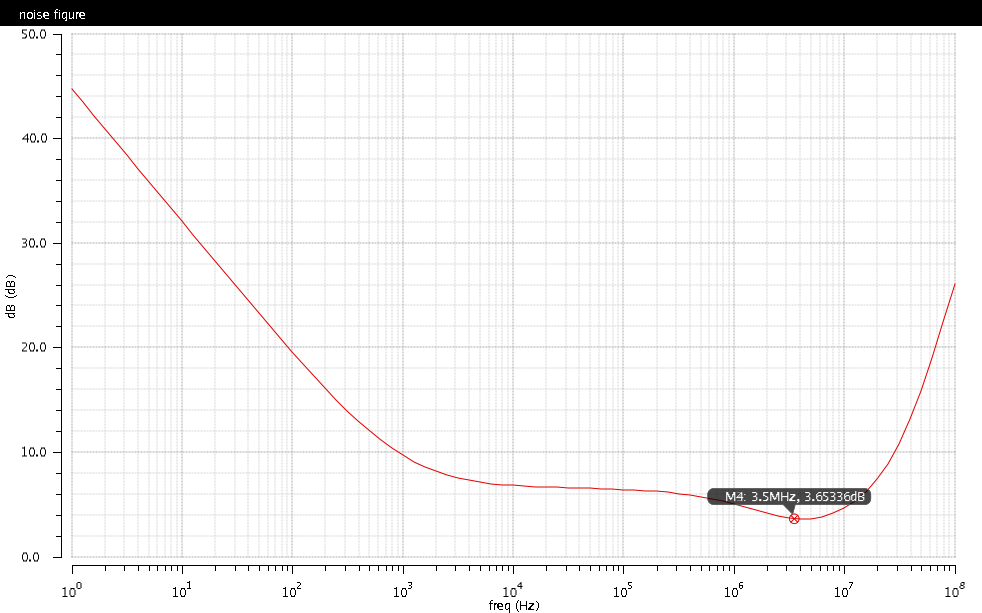
\includegraphics[width=0.5\textwidth]{figures/FullSysNoiseFigure.png}
    \caption{Full system noise due to LNA and Mixer}
    \label{fig:fullsystemnoise}
\end{figure}

The overall linearity of the system is about {\bf -31 dBm} however a graph is not shown due to technical issues with the Cadence software. Overall the full system results can be found in TABLE ~\ref{tab:systemresults}.


\begin{table}[h]
\begin{center}
	\begin{tabular}{ |c | c | }
 		\hline                      
  		Conversion gain & 35.92 dB \\ \hline
  		Noise Figure & 3.65 dB \\ \hline
  		IIP3 & -31 dBm\\ \hline
		Total power & 1.8mW \\
  		\hline  
	\end{tabular}

\end{center}
\caption{Final results from system integration}
\label{tab:systemresults}
\end{table}
